
\section{Direct Evaluation: Ranking Word Pairs}

\begin{figure*}[th!]
\begin{center}
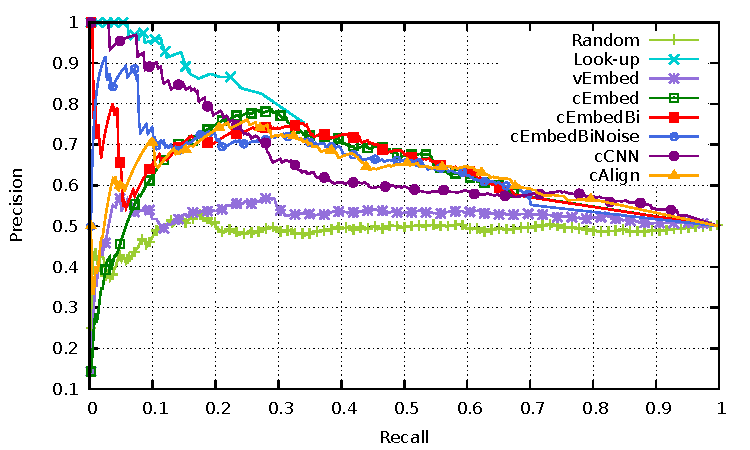
\includegraphics[width=\textwidth]{mainmatter/emnlp2016-causal/direct2.pdf} % {rpcurves_all.png}
%space{-3mm}
\caption{{\footnotesize Precision-recall curve showing the ability of each model to rank causal pairs above non-causal pairs. For clarity, we do not plot cEmbedNoise, which performs worse than cEmbedBiNoise. The Look-up model has no data points beyond the 35\% recall point.}}
%space{-4mm}
\label{fig:rpcurve_all}
\end{center}
\end{figure*}

%\flushleft{\textbf{Results:}} 

\label{sec-emnlp2016:directeval}

%Before we discuss the utility of these models for causal QA, we implement a {\em direct} evaluation
We begin the assessment of our models with a {\em direct} evaluation to determine whether or not the proposed approaches capture causality better than general-purpose word embeddings and whether their robustness improves upon a simple database look-up.
For this evaluation, we follow the protocol of Levy and Goldberg~\citeyear{levy2014dependency}.  
In particular, we create a collection of word pairs, half of which are causally related, with the other half consisting of other relations. 
These pairs are then ranked by our models and several baselines, with the goal of ranking the causal pairs above the others. 
The embedding models rank the pairs using the cosine similarity between the target vector for the causal word and the context vector of the effect word.  The alignment model ranks pairs using the probability $P(\text{Effect}|\text{Cause})$ given by IBM Model 1, and the CNN ranks pairs by the value of the output returned by the network.
%To demonstrate that their embeddings encoded functional similarity rather than relatedness, they ranked a set of word pairs (each of which reflected one of the two types of similarity) using cosine similarity and showed that the word pairs which were functionally similar tended to be ranked higher than those with topical similarity.  Here, we do the same.

%\flushleft{\textbf{Data:}} 
\subsection{Data}
In order to avoid bias towards our extraction methods, we evaluate our models on an external set of word pairs drawn from the SemEval 2010 Task 8 \cite{hendrickx2009semeval}, originally a multi-way classification of semantic relations between nominals.  We used a total of 1730 nominal pairs, 865 of which were from the Cause-Effect relation (e.g., (\emph{dancing $\rightarrow$ happiness})) and an equal number which were randomly selected from the other eight relations (e.g., (\emph{juice $\rightarrow$ grapefruit}), from the Entity-Origin relation).  This set was then randomly divided into equally-sized development and test partitions.

%\flushleft{\textbf{Baselines:}} 
\subsection{Baselines}
We compared our distributional similarity models against three baselines:

{\flushleft \textbf{Vanilla Embeddings Model (vEmbed):}} a standard \texttt{word2vec} model trained with the skip-gram algorithm and a sliding window of 5, using the original texts from which our causal pairs were extracted.\footnote{All embedding models analyzed here, including this baseline and our causal variants, produced embedding vectors of 200 dimensions.} As with the cEmbed model, SemEval pairs were ranked using the cosine similarity between the vector representations of their arguments.
%space{-1mm}

{\flushleft \textbf{Look-up Baseline:}} a given SemEval pair was ranked by the number of times it appeared in our extracted cause-effect tuples. 
%space{-1mm}

{\flushleft \textbf{Random:}} pairs were randomly shuffled.
%space{-1mm}



%%
%% MAP Table 
%%
%\begin{table}[t!]
%\begin{center}
%%\begin{scriptsize}
%\begin{footnotesize}
%\begin{tabular}{ll}
%\hline
%\multicolumn{1}{l}{ Model } & \multicolumn{1}{l}{MAP} \\ %\multicolumn{1}{l}{Impr.} \\
%%\cline{1-2}
%\hline
%%\multicolumn{2}{l}{\textit{Yahoo! Answers}} \\ % 185q (sent) ret=1p c=0.1 
%%\hline
%Random 			& 48.8 	\\
%Look-up			& 63.1$^*$ 	\\
%vEmbed 			& 52.5	\\
%cEmbed  			& 60.8$^*$	\\
%cEmbedBi	                & 62.8$^*$	\\
%cEmbedNoise           & 62.0$^*$	\\ 
%cEmbedBiNoise        & 63.6$^*$	\\ 
%cAlign  			& 61.6$^*$  \\
%cCNN  			& 67.5$^*$	\\
%\end{tabular}
%\end{footnotesize}
%\caption{{\footnotesize Performance in the direct evaluation, measured with mean average precision (MAP).  The ``Bi'' suffix indicates a bidirectional model; the ``Noise'' suffix indicates a model that is noise aware. $^*$  indicates that the difference between the corresponding model and vEmbed is statistically significant ($p < 0.05$), %. Statistical significance was 
%as determined through a one-tailed bootstrap resampling test with 10,000 iterations.}} 
%\label{tab:MAP}
%\vspace{-4mm}
%\end{center}
%\end{table}
%%MAP for Custom Vectors: 0.6816675505751166
%%MAP for E2C Vectors: 0.6871338630607531
%%MAP for Bidir Vectors: 0.6684350003582593
%%MAP for Comparison (Baseline) Vectors: 0.5835158858435683
%%MAP for Translation Model with lamda of 0.5 : 0.6156522257806402
%%MAP for counting Matches: 0.9312613087523468
%%MAP for Keras: 0.6752727545259546
%%MAP for Random: 0.4892479543525109
%%p < 0.01


\subsection{Results}

Figure \ref{fig:rpcurve_all} shows the precision-recall (PR) curve for each of the models and baselines. 
As expected, the causal models are better able to rank causal pairs than the vanilla embedding baseline (vEmbed), which, in turn, outperforms the random baseline.  Our look-up baseline, which ranks pairs by their frequency in our causal database, shows a high precision for this task, but has coverage for only 35\% of the causal SemEval pairs.
%This demonstrates that it is beneficial to have custom models for the semantic relation of interest. 
%First, all the proposed models perform better than the vanilla embedding baseline (vEmbed), which, in turn, outperforms the random baseline. 
%The difference between all our proposed causal models and the vEmbed baseline is statistically significant. 
%

Some models perform better on the low-recall portion of the curve (e.g., the look-up baseline and cCNN), while the embedding and alignment models have a higher and more consistent performance across the PR curve. We hypothesize that models that better \emph{balance} precision and recall will perform better in a real-world QA task, which may need to access a given causal relation through a variety of lexical patterns or variations. We empirically validate this observation in Section~\ref{sec-emnlp2016:indirecteval}.

%, suggesting that causal embedding models may be more practical in a real-world QA system than cCNN. We empirically validate this intuition in Section. 

%perform better in the mid-low recall portion of the curve (e.g. cEmbedBi).  This is well-illustrated by the look-up baseline, which has high precision in the low-recall portion of the curve, but which only has coverage of 35\% of the causal SemEval pairs.  
%The cCNN model outperforms the cEmbed and cAlign models for the low-recall part of the curve (which explains why cCNN has the highest overall MAP). But the latter models 


%Second, the look-up baseline has a higher MAP than several of the causal models, despite having coverage of only 35\% of the causal SemEval pairs.  This suggests that the MAP score is dominated by precision, rather than recall.
%Despite the high overall MAP, this lack of coverage renders this an impractical model, because a real-world QA system is more likely to encounter questions that are lexically different than the pairs in our database. 


%Second, we see that models which had higher MAP demonstrate higher precision in the low-recall portion of the curve, while the models which perform better in the mid-low recall portion of the curve have slightly lower MAPs.  
%This is well-illustrated by the Look-up baseline, whose MAP is higher than many of the causal models, and which has excellent precision in the low-recall portion of the curve, but which only provides coverage for 35\% of the causal pairs.  
%We hypothesize that is the models that better balance precision and recall that will perform well in a real-world QA system, where it is more likely that questions will be lexically different than the pairs in our database.


%Second, somewhat disturbingly, the look-up baseline seemingly outperforms most of the embedding models. 

%However, this score is highly skewed by the fact that approximately 35\% of the causal SemEval pairs were also found in our casual database, and were scored with high precision due to the direct evidence available. However, the remaining pairs received a score of 0. 

%% WHAT IT JUST WAS:
%However, this score is highly skewed: 35\% of the causal SemEval pairs were also found in our casual database, and so were scored with high precision due to the direct evidence available, but the remaining 65\% of pairs all received a score of 0.
%Despite the high overall MAP, this lack of coverage renders this an impractical model, because a real-world QA system is more likely to encounter questions that are lexically different than the pairs in our database. 

%Thus, the MAP score for this model is unrealistically skewed.
% \todo{Say something about how these evaluations are not ideal}~\cite{faruqui2016problems}.

%the high precision of pairs which are found in the database coupled with the very low recall (only 35\% of the pairs were found in the extracted pairs), resulting in the majority of the pairs being tied in the lowest rank, skewing the average.
%that when pairs are found, there is extremely high confidence that they are of the relation of interest coupled with the fact that approximately 65\% of the pairs were not found in the database and so were all tied in last place.  
%As a consequence, there were far fewer average precisions to be combined when calculating the MAP, and most of the ones which were there had extremely high precision.  
% The MAP when using the customized vectors was significantly higher than that of the standard \texttt{word2vec} vectors (68\% versus 58\%, $p<0.01$), and both were higher than the baseline ().  %This suggests that while the standard implementation of \texttt{word2vec} encodes some causality information, our method encodes it far more directly. \todo{better word}.

% \subsection{Discussion}
%To better understand these models, we plot the precision-recall (PR) curve in Figure \ref{fig:rpcurve_all}. 
%The curve highlights the issue discussed above: the look-up model ranks a few pairs with high precision, but does not address the majority of the data. 
%Conversely, the proposed causal models consistently outperform the vEmbed baseline for the high-recall portion of the curve.



The PR curve for the causal embeddings shows an atypical dip at low-recall.  To examine this, we analyzed its top-ranked 15\% of SemEval pairs, and found that incorrectly ranked pairs were not found in the database of causal tuples.  Instead, these incorrect rankings were largely driven by low frequency words whose embeddings could not be robustly estimated due to lack of direct evidence.  
%\todo{Optional: I know we're low on space, but the example that Becky had here was great. Any way to put it back?}
Because this sparsity is partially driven by directionality, 
we implemented a bidirectional embedding model (cEmbedBi) that (a) trains a second embedding model by reversing the input (effects as targets, causes as contexts), and (b) ranks pairs by the \textit{average} of the scores returned by these two unidirectional causal embedding models. 
Specifically, the final bidirectional score of the pair, $(e_1, e_2)$, where $e_1$ is the candidate cause and $e_2$ is the candidate effect, is:
\begin{equation}
s_{bi}(e_1, e_2) = \tfrac{1}{2}(s_{c{\rightarrow}e}(e_1, e_2) + s_{e \rightarrow c}(e_2, e_1))
\end{equation}
where $s_{c \rightarrow e}$ is the score given by the original causal embeddings, i.e., from cause to effect, and $s_{e \rightarrow c}$ is the score given by the reversed-input causal embeddings, i.e., from effect to cause.

As Figure~\ref{fig:rpcurve_all} shows, the bidirectional embedding variants consistently outperform their unidirectional counterparts. 
All in all, the best overall model is cEmbedBiNoise, which is both bidirectional and incorporates the noise handling approach from Section~\ref{sec-emnlp2016:models}. This model substantially improves performance in the low-recall portion of the curve, while also showing strong performance across the curve. 



%
%The curve for the customized vectors shows an atypical shape in its low-recall part.
%Here, the highest ranked pairs had \emph{worse} precision rather than the expected higher precision.  To examine this, we analyzed the top-ranked 15\% of the pairs from the ranking produced by  the causal vectors.  
%%
%Our analysis found that these pairs tend to be incorrectly ranked because the cEmbed model performs a form of soft approximate inference (which was our goal!), but which backfired on these data points.  For example, the top-ranked (incorrect) pair was \emph{platform} $\rightarrow$ \emph{scaffold}, and there were no instances in our causal database where \emph{platform} and \emph{scaffold} were found together in the same cause-effect pair.  
%%
%Instead, we found that there were  three other extracted tuples with \emph{scaffold} in the effect text. Further, these tuples had other effects  that overlapped lexically with effects of \emph{platform}, which ``pulled'' \emph{platform} closer to \emph{scaffold}.  For example, a phrase containing \emph{malfunction} 
%shares {\em loss} as a common effect with \emph{platform}, and \emph{malfunction} has other effects that contain \emph{scaffold}. 
%In general, we found that these examples of semantic drift~\cite{curran2007minimising} occur for low frequency data, where neither the direct evidence nor the embeddings are robustly estimated. 
%
%%cause \emph{loss}, which brings these two words closer in the target embedding space.
%%%, since they have similar effects.  
%%This resulted in \emph{platform}'s effects being close to the effects of \emph{malfunction}, which include \emph{scaffold}.  This demonstrates that the inference is influenced by frequency effects, as words like \emph{scaffold} and \emph{platform} are too infrequent to have robust representations in the embedding space.  
%%\todo{This last sentence needs better explanation: why does this happen only at low-recall?}
%
%As this semantic drift effect is entirely directional, we implemented a bidirectional embedding approach, which: (a) trains a second embedding model by reversing the input, such that the effects served as the targets and the causes were the contexts, and (b) 
%ranks pairs by the average of the scores returned by the two causal embeddings. As Table~\ref{tab:MAP} and Figure~\ref{fig:rpcurve_all} show, the bidirectional embedding variants consistently outperform their unidirectional counterparts. cEmbedBiNoise, which incorporates the noise handling approach from Section~\ref{sec-emnlp2016:models} and is bidirectional, resolves the dip in low-recall part of the curve, and outperforms cCNN for most of the data. 
%
%%As this effect is entirely directional, we trained a set of vectors by reversing the input, such that the effects served as the targets and the causes were the contexts.  The precision-recall curve when using these embeddings to rank the SemEval pairs is shown in Figure \ref{fig:rpcurve_all}, labelled as E2C.  As expected, the curve follows that of the original vectors, as it suffers from the same issues, but with different noisy pairs ranked highly.  We then ranked the SemEval pairs using an average of the scores returned by the two causal embeddings, to mitigate the frequency effects.  That final, bidirectional curve is also shown in Figure \ref{fig:rpcurve_all}.
%%Instead, we found that many of the causal events which whose cause argument contained the word \emph{platform} had effects which overlapped lexically with those whose cause arguments contained the word \emph{malfunction}, and that there w.  To illustrate, consider the following sentences 
%%we had several extracted causal events whose cause contained the word \emph{platform} and whose effect contained the words \emph{}
%

